\documentclass[main.tex]{subfiles}

\begin{document}
	
	\section{Постановка задачи}
	Найти минимум функции методами одномерной минимизации (метод золотого сечения и метод Фибоначчи)\\
	Необходимо подтвердить унимодальность функции построением графика.\\
	Предусмотреть счётчик числа обращений к функции.
	Произвести вычисления с точностью: десятая, сотая, тысячная.
	Вывести формулу связи обращений к функции и заданной функции
	\section{Исследование применимости метода}
	Метод Фибоначчи является улучшением метода золотого сечения. Метод отличается от метода золотого сечения тем, что коэффициент сокращения интервала неопределенности меняется от итерации к итерации.\\
	Для того, чтобы оба метода были применимы необходима унимодальность исследуемой функции (подтверждение унимодальности - график(\ref{function2})). Иначе мы можем прийти в локальный минимум и на этом процесс остановится.
	\newpage
	\section{Описание алгоритмов методов}
	\subsection{Метод золотого сечения}
	\begin{algorithm}[H]\label{golden_ratio}
		\KwData{$f, a, b, \epsilon$ -- исследуемая на экстремум функция; границы интервала унимодальности функции, где ищется экстремум; точность - величина, которую не должна превышать длина интервала неопределенности.}
		
		\KwResult{интервал неопределенности -- подынтервал интервала $[a, b]$, содержащий min и такой, что его длина не превосходит $\epsilon$.}
		
		$\alpha = \frac{3-\sqrt{5}}{2}$ ($\alpha = \frac{1}{\phi^2}$, где $\phi$ -- золотое сечение)\;
		\If{$b - a \leq eps$} {return $[a, b]$}
		$a_k = a, b_k = b$ - текущий интервал поиска min\;
		$interval\_length = b_k - a_k$\;
		$\lambda_k = a_k + \alpha\cdot interval\_length$\;
		$\mu_k = b_k - \alpha\cdot interval\_length$\;
		$f_{\lambda_k} = f(\lambda_k)$\;
		$f_{\mu_k} = f(\mu_k)$\;
		\While{$interval\_length > \epsilon$}{
			\If{$f_{\lambda_k} < f_{\mu_k}$}{
				$b_k = \mu_k$\;
				$\mu_k = \lambda_k$\;
				$f_{\mu_k} = f_{\lambda_k}$\;
				$interval\_length = b_k - a_k$\;
				$\lambda_k = a_k + \alpha * interval\_length$\;
				$f_{\lambda_k} = f(\lambda_k)$\;
			}\Else{
				$a_k = \lambda_k$\;
				$\lambda_k = \mu_k$\;
				$f_{\lambda_k} = f(\lambda_k)$\;
				$interval\_length = b_k - a_k$\;
				$\mu_k = b_k - \alpha\cdot interval\_length$\;
				$f_{\mu_k} = f(\mu_k)$\;
			}		
		}
		\If{$f_{\lambda_k} < f_{\mu_k}$}{return $[a_k, \mu_k]$}
		return $[\lambda_k, b_k]$\;		
		\caption{Метод золотого сечения}
	\end{algorithm}
	Замечание: Для контроля количества обращений к функции была написана функция-декоратор. Декоратор считает количество вызовов функции и записывает в атрибут ncalls. 
	
	
	
	\subsection{Метод Фибоначчи}
	\begin{enumerate}
		\item Выбираем допустимую конечную длину интервала неопределенности l и константу различимости $\epsilon$ 
		\item Выбираем общее число вычислений функции n так, что $F_n >\frac{b-a}{l}$
		\item Положим $\lambda_1 = a_1+\frac{F_{n-2}}{F_n}(b-a)$ и  $\mu_1 = a_1+\frac{F_{n-1}}{F_n}(b-a)$
		\item Вычислим значения функции в точках $\lambda_1$ и $\mu_1$
		\item Положим k = 1
		\item Если значение функции в точке $\lambda_k$ больше, чем в точке $\mu_k$ перейдем к пункту 7, иначе к пункту 8
		\item Положим $a_{k+1} = \lambda_k$, $b_{k+1} = b_k$, $\lambda_{k+1} = \mu_k$, $\mu_{k+1} = a_{k+1}+\frac{F_{n-k-1}}{F_{n-k}}(b_{k+1}-a_{k+1}$\\
		Если k = n - 2, то перейдем к пункту 10, иначе вычисляем функцию в точке $\mu_{k+1}$ и переходим к пункту 9
		\item Положим $a_{k+1} = a_k$, $b_{k+1} = \mu_k$, $\mu_{k+1} = \lambda_k$, $\lambda_{k+1} = a_{k+1}+\frac{F_{n-k-2}}{F_{n-k}}(b_{k+1}-a_{k+1}$\\
		Если k = n - 2, то перейдем к пункту 10, иначе вычисляем функцию в точке $\mu_{k+1}$ и переходим к пункту 9
		\item Заменяем k на k+1 и переходим к пункту 6
		\item Положим $\lambda_{n} = \lambda_{n-1}$, $\mu_{n} = \lambda_n + \epsilon$. Если функция в точке $\lambda_n$ равна функции в точке $\mu_n$, то положим $a_n = \lambda_n$, $b_n=b_{n-1}$, иначе $a_n = a_{n-1}$, $b_n=\mu_n$. Повторяем пока заданный интервал неопределенности не удовлетворяет заданной точности.
	\end{enumerate}
	
	\section{Результаты решения задачи}
	Рассмотрим функцию \newline$f(x) = sin(\pi x) + cos(\pi x)$ на промежутке ее унимодальности $[a, b] = [0, 2].$\\
	
	\begin{table}[h]
		\begin{tabular} { | p{0.1\linewidth} | p{0.25\linewidth} | p{0.45\linewidth} |}
			\hline
			$\epsilon$ & число обращений & длина интервала неопределенности  \\ \hline
			0.1 & 9 & 0.04  \\ \hline
			0.01 & 14 & 0.004  \\ \hline
			0.001 & 18 & 0.0006   \\ \hline
		\end{tabular}
		\caption{Метод Золотого сечения.}
	\end{table}
	
	\begin{table}[h]
		\begin{tabular} { | p{0.1\linewidth} | p{0.25\linewidth} | p{0.45\linewidth} |}
			\hline
			$\epsilon$ & число обращений & длина интервала неопределенности  \\ \hline
			0.1 & 9 & 0.06  \\ \hline
			0.01 & 14 & 0.005 \\ \hline
			0.001 & 19 &  0.0005  \\ \hline
		\end{tabular}
		\caption{Метод Фибоначчи.}
	\end{table}
	
	
	\section{Оценка достоверности полученного результата}
	Найдем аналитически минимум путем дифференцирования:
	$f(x) = sin(\pi x) + cos(\pi x), [a, b] = [0, 2] \rightarrow x_{min} = 1.25.$
	Подтвердим результат графически:
	\begin{figure}[H]
		\center{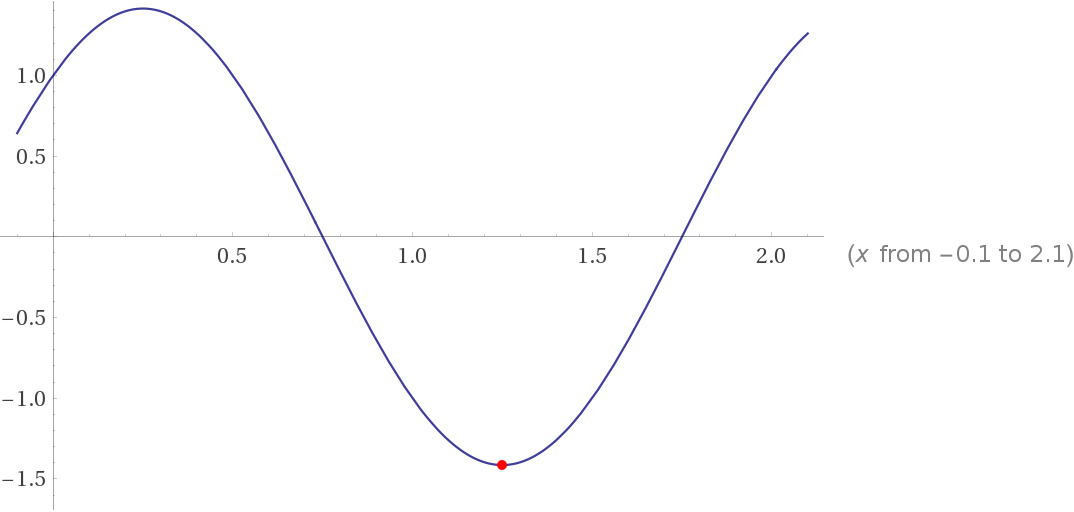
\includegraphics[width=.7\textwidth]{img/2.jpg}}
		\caption{$f(x) = sin(\pi x) + cos(\pi x)$}
		\label{function2}
	\end{figure}
	Убедимся, что истинный минимум на промежутке действительно принадлежит интервалам неопределенности для всех исследуемых значений $\epsilon$.\\
	
	\begin{table}[h]
		\begin{tabular} { | p{0.1\linewidth} | p{0.35\linewidth} |}
			\hline
			$\epsilon$ &  интервал неопределенности  \\ \hline
			0.1 & [1.24 1.28]   \\ \hline
			0.01 & [1.248 1.252] \\ \hline
			0.001 & [1.2497 1.2503]    \\ \hline
		\end{tabular}
		\caption{Метод Золотого сечения, интервалы неопределенности.}
	\end{table}
	
	
	\begin{table}[h]
		\begin{tabular} { | p{0.1\linewidth} | p{0.35\linewidth} |}
			\hline
			$\epsilon$ &  интервал неопределенности  \\ \hline
			0.1 & [1.23, 1.29]   \\ \hline
			0.01 & [1.252, 1.257] \\ \hline
			0.001 & [1.2499 1.2504]    \\ \hline
		\end{tabular}
		\caption{Метод Фибоначчи, интервалы неопределенности.}
	\end{table}
	$x_{min}$ лежит в полученных интервалах неопределенности -- методы работают корректно!
	
	\begin{thebibliography}{99}
		
	\end{thebibliography}
	
	
\end{document}
